\par
Graficzny interfejs użytkownika został zaimplementowany za pomocą klasy \qtclass{QWidget}.
Klasa ta dziedziczy po \qtclass{QObject} i po \qtclass{QPaintDevice}, obiekcie służącym do rysowania.
\qtclass{QWidget} reprezentuje element graficzny interfejsu użytkownika, ma zaimplementowany mechanizm renderowania, wyświetlania na ekranie użytkownika, obsługi myszki klawiatury, przeciągnięcia i upuszczenia \fromEng{drag and drop}, itp.
Wszystkie elementy takie jak przyciski i pola tekstowe muszą dziedziczyć po niej.
\par
Interfejs klasy jest niezależny od platformy, na której się znajduje.
Nawet tworzenie własnej, niestandardowej kontrolki nie wymaga uwzględniania systemu operacyjnego, a przynajmniej w kwestii użytkowej.

\begin{figure}[!htbp]
    \centering
    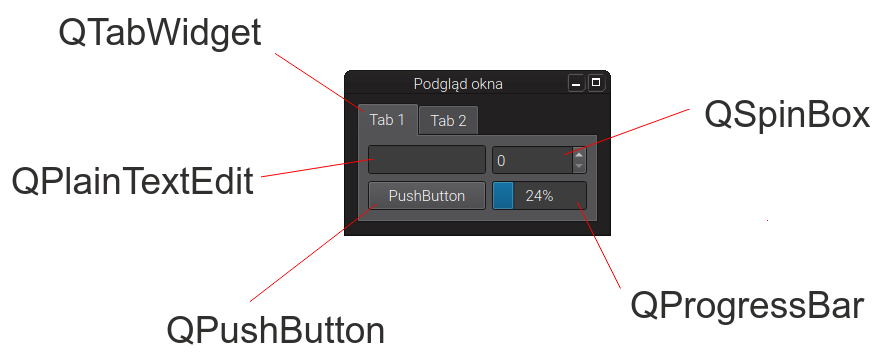
\includegraphics[width=\textwidth]{img/qt-gui-001.png}
    \caption{Przykładowe okienko programu w Qt. Zdjęcie własne.}
    \label{fig:qtgui1}
\end{figure}

\par
Kilka przykładowych klas obiektów graficznych i ich cechy:
\begin{itemize}
    \item \qtclass{QLabel} --- klasa służąca do wyświetlania tekstu bez możliwości interakcji z nim.
          Dziedziczy po klasie \qtclass{QFrame}, która dziedziczy po \qtclass{QWidget}.

    \item \qtclass{QPushButton} --- klasa do tworzenia zwykłego przycisku.
          Dziedziczy po klasie \qtclass{QAbstractButton}, która dziedziczy po \qtclass{QWidget}.
          Obsługa zdarzenia wciśnięcia przycisku jest przez obsługę sygnału \qtfunction{QAbstractButton}{clicked}.
          Przykład można zobaczyć na rysunku \ref{fig:qtgui1}.

    \item \qtclass{QTabWidget} --- implementuje zakładki, takie jak w przeglądarce internetowej.
          Dziedziczy bezpośrednio po klasie \qtclass{QWidget}.
          Zawartości zakładek mogą być zwykłymi obiektami dziedziczącymi po \qtclass{QWidget}.
          Przykład można zobaczyć na rysunku \ref{fig:qtgui1}.

    \item \qtclass{QPlainTextEdit} --- implementuje pole umożliwiające wprowadzanie teksu rzez użytkownika.
          Dziedziczy po klasie \qtclass{QAbstractScrollArea}, które dziedziczy po  \qtclass{QFrame}, z kolei ta po \qtclass{QWidget}.
          Przykład można zobaczyć na rysunku \ref{fig:qtgui1}.

    \item \qtclass{QProgressBar} --- implementuje pasek postępu w dwóch wersjach poziomej i pionowej.
          Dziedziczy bezpośrednio po klasie \qtclass{QWidget}.
          Przykład poziomego paska można zobaczyć na rysunku \ref{fig:qtgui1}.

    \item \qtclass{QSpinBox} --- implementuje prządkę, czyli kontrolkę przystosowaną do wprowadzania liczb przez użytkownika.
          Posiada dwa dodatkowe przyciski pozwalające w łatwy sposób zwiększyć lub zmniejszyć zawartość.
          Przykład można zobaczyć na rysunku \ref{fig:qtgui1}.

\end{itemize}